\subsection*{Cuñas - Anillos de Newton}

\item Una cuña de aire es iluminada de tal forma que si incide luz de longitud de onda \(\lambda = \SI{5000}{\angstrom}\) normalmente a la cara inferior, produce
franjas paralelas cuya distancia entre mínimos es \SI{1}{\milli\metre}.
Describir la cuña. 


\item Se observan anillos de Newton por reflexión, iluminándose una lente plano--convexa con luz de longitud de onda \(\lambda = \SI{650}{\nano\metre}\).
¿Qué radio de curvatura tiene la lente si el segundo anillo oscuro tiene \(d = \SI{2.6}{\milli\metre}\) de diámetro? 



\item
\begin{minipage}[t][4.8cm]{0.65\textwidth}
Se observan anillos de Newton mediante una lámina de vidrio de índice de refracción $n_3$, una lente de vidrio con $n_1 \ne n_3$ y un líquido de $n_2$ intermedio entre $n_1$ y $n_3$ (ver figura). 
\begin{enumerate}
\item ¿Son oscuros o brillantes los centros del sistema de anillos observados respectivamente por reflexión y transmisión? 
\item Suponga ahora que el líquido tiene un índice $n_2 = \num{1.59}$.
Si se observan los anillos por reflexión siendo $\lambda = \SI{5900}{\angstrom}$, y el radio del quinto anillo es de \SI{2}{\milli\metre}, ¿cuál es el radio de curvatura
de la lente?
\end{enumerate}
\end{minipage}
\begin{minipage}[c][0cm][t]{0.3\textwidth}
	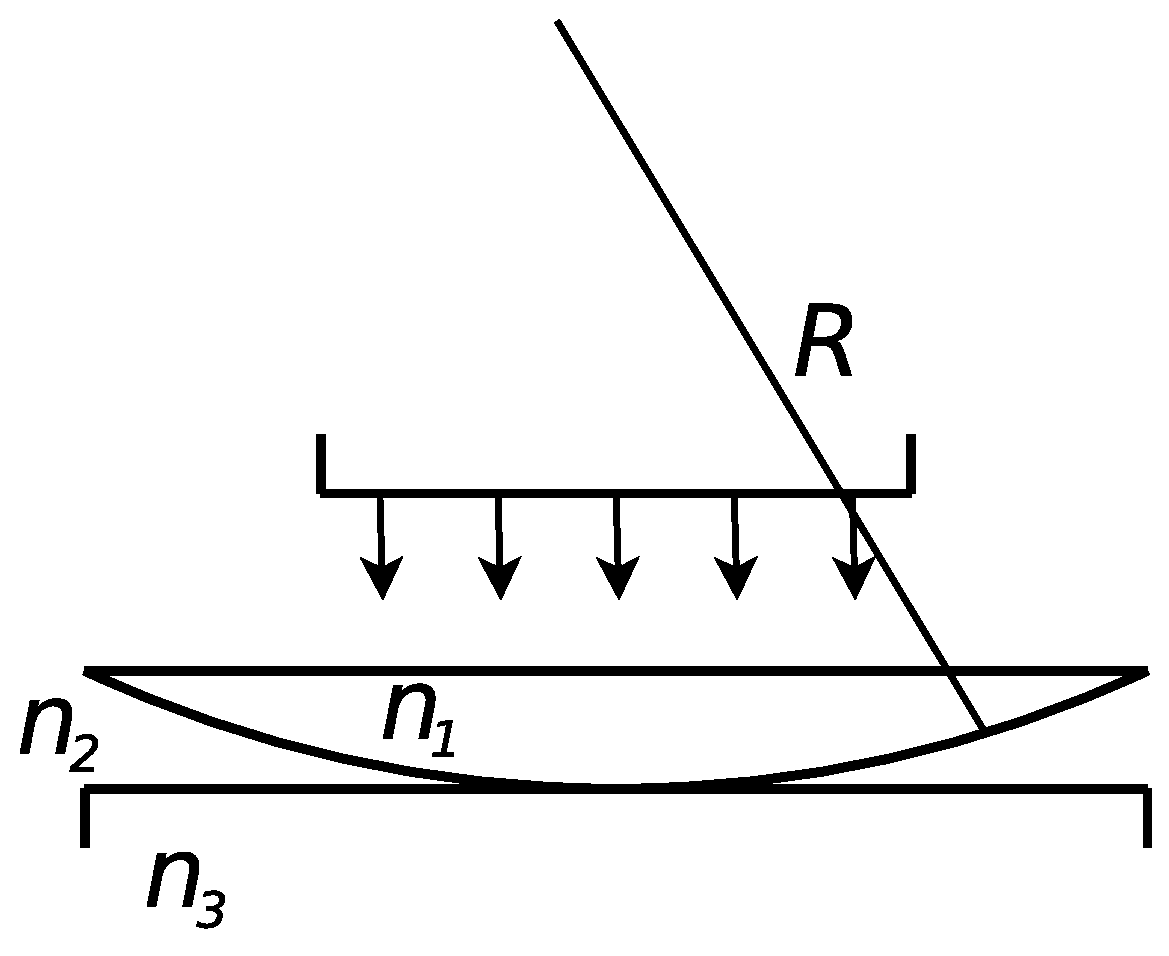
\includegraphics[width=\textwidth]{ej5-26}
\end{minipage}



\item Se observan anillos de Newton con una lente plano--convexa situada sobre un vidrio plano, con aire entre medio.
¿Qué pasa con la diferencia entre los cuadrados de dos radios consecutivos si: 
\begin{enumerate}
	\item Se cambia la lente por otra también plano-convexa del mismo radio de curvatura, pero de mayor índice de refracción? 
	\item Se coloca agua en vez de aire entre la lente y la lámina de vidrio? 
\end{enumerate}



\item Con el mismo dispositivo de los problemas anteriores se observan anillos de Newton por reflexión.
¿Es oscuro o claro el centro de la figura de interferencia?
¿Cuál es el radio del tercer anillo brillante?
¿Qué sucede con los anillos para un ligerísimo desplazamiento hacia arriba de la lente: convergen hacia el centro o se alejan de éste?
¿Por qué? 
Datos: $R = \SI{1}{\metre}$; $d = \SI{0.013}{\milli\metre}$; $\lambda = \SI{5000}{\angstrom}$; $n_1 = \num{1.5}$; $n_2 = \num{1.3}$; $n_3 = \num{1.4}$.



\item En un dispositivo para observar anillos de Newton el espacio entre la lente y la lámina de vidrio está lleno de líquido.
Se observan anillos por transmisión.
La longitud de onda empleada es $\lambda = \SI{5890}{\angstrom}$ y el radio de curvatura de la lente es de \SI{10}{\metre}.
Hallar el índice de refracción del líquido sabiendo que el radio del tercer anillo brillante es de \SI{3.65}{\milli\metre}.



\item
\begin{minipage}[t][0cm]{0.65\textwidth}
Considere el dispositivo de anillos de Newton modificado que se muestra en la figura.
Se observan anillos por reflexión. 
\end{minipage}
\begin{minipage}[c][2.2cm][t]{0.3\textwidth}
	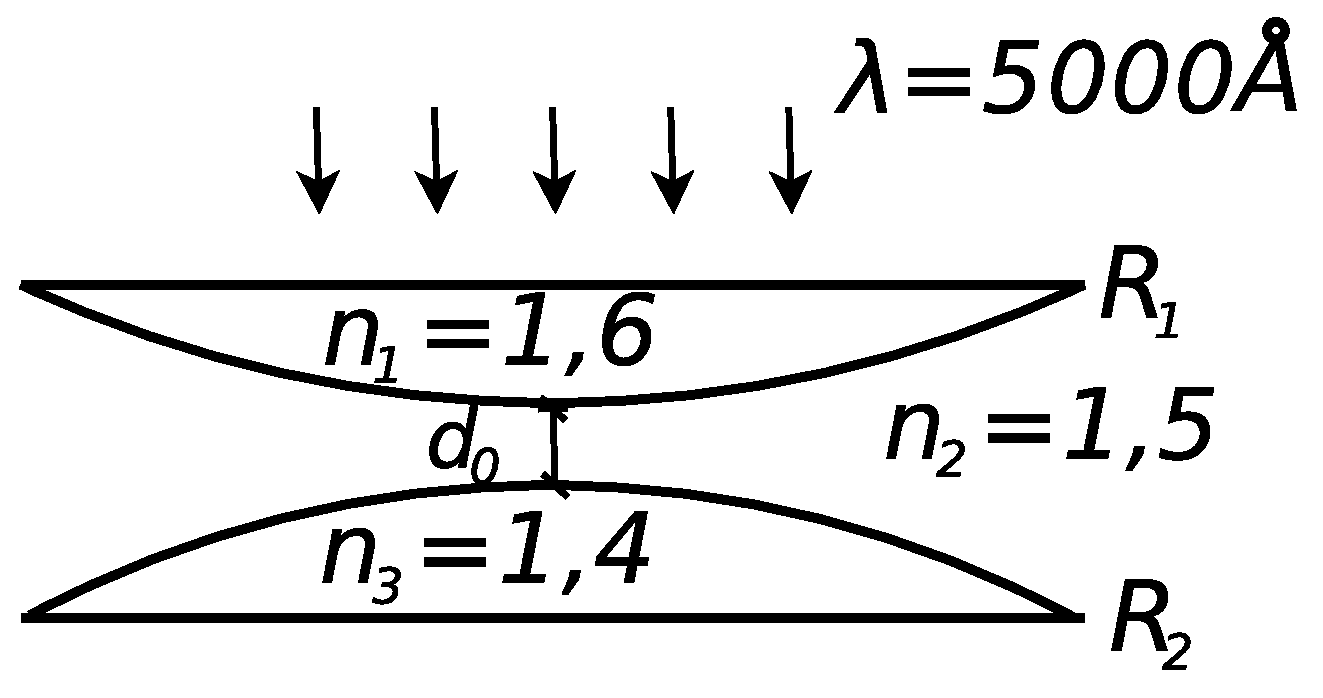
\includegraphics[width=\textwidth]{ej5-30}
\end{minipage}
\begin{enumerate}
	\item ¿Para qué valores de $d_0$ el centro de los anillos corresponde a un máximo? 
	\item Hallar el mínimo valor de $d_0$ para el cual el centro de los anillos corresponde a un mínimo. 
	\item Con el valor de $d_0$ hallado en b), calcular la relación que debe existir entre los radios de las lentes, $R_2 = R_2(R_1)$, para que el radio del primer anillo oscuro verifique $r_1^2 = \SI{e+15}{\angstrom\squared}$
\end{enumerate}
